\documentclass[a4paper]{article} 
\addtolength{\hoffset}{-2.25cm}
\addtolength{\textwidth}{4.5cm}
\addtolength{\voffset}{-3.25cm}
\addtolength{\textheight}{5cm}
\setlength{\parskip}{3pt}
\setlength{\parindent}{0in}

%----------------------------------------------------------------------------------------
%	PACKAGES AND OTHER DOCUMENT CONFIGURATIONS
%----------------------------------------------------------------------------------------

\usepackage{charter} % Use the Charter font
\usepackage[utf8]{inputenc} % Use UTF-8 encoding
\usepackage{microtype} % Slightly tweak font spacing for aesthetics
\usepackage[english, ngerman]{babel} % Language hyphenation and typographical rules
\usepackage{amsthm, amsmath, amssymb} % Mathematical typesetting
\usepackage{float} % Improved interface for floating objects
\usepackage{hyperref, xurl} % For hyperlinks in the PDF
\usepackage{graphicx, multicol} % Enhanced support for graphics
\usepackage{xcolor} % Driver-independent color extensions
\usepackage{marvosym, wasysym} % More symbols
\usepackage{rotating} % Rotation tools
\usepackage{censor} % Facilities for controlling restricted text
\usepackage{listings, style/lstlisting} % Environment for non-formatted code, !uses style file!
%\usepackage{pseudocode} % Environment for specifying algorithms in a natural way
\usepackage{algorithm}
\usepackage{algorithmic}
\usepackage{array}
\usepackage{multirow}
\usepackage{makecell}
\usepackage{pdfpages}
%\usepackage{style/avm} % Environment for f-structures, !uses style file!
\usepackage{booktabs} % Enhances quality of tables
\usepackage{tikz-qtree} % Easy tree drawing tool
\tikzset{every tree node/.style={align=center,anchor=north},
         level distance=2cm} % Configuration for q-trees
%\usepackage{style/btree} % Configuration for b-trees and b+-trees, !uses style file!
\usepackage[backend=biber,style=numeric,
            sorting=nyt]{biblatex} % Complete reimplementation of bibliographic facilities
\addbibresource{ecl.bib}
\usepackage{csquotes} % Context sensitive quotation facilities
%\usepackage[yyyymmdd]{datetime} % Uses YEAR-MONTH-DAY format for dates
%\renewcommand{\dateseparator}{-} % Sets dateseparator to '-'
\usepackage{fancyhdr} % Headers and footers
\pagestyle{fancy} % All pages have headers and footers
\fancyhead{}\renewcommand{\headrulewidth}{0pt} % Blank out the default header
\fancyfoot[L]{} % Custom footer text
\fancyfoot[C]{} % Custom footer text
\fancyfoot[R]{\thepage} % Custom footer text
\newcommand{\note}[1]{\marginpar{\scriptsize \textcolor{red}{#1}}} % Enables comments in red on margin

\newcommand{\classname}[1]{\texttt{#1}}
\newcommand{\highlight}[1]{\textbf{#1}}

\long\def\citacao#1{\medskip % \citacao is the command
	\begingroup
	\parindent 0pt
	\leftskip=1.27cm
	\small #1 \par \medskip
	\endgroup
}
%----------------------------------------------------------------------------------------

\begin{document}

%-------------------------------
%	TITLE SECTION
%-------------------------------

\fancyhead[C]{}
\hrule \medskip % Upper rule
\begin{minipage}{0.295\textwidth} 
\raggedright
\footnotesize
Robert Roth \hfill\\   
Sommersemester 2025\hfill\\  
\end{minipage}
\begin{minipage}{0.4\textwidth} 
\centering 
\large 
Übung 01\\ 
\normalsize 
Spieleprogrammierung\\ 
\end{minipage}
\begin{minipage}{0.295\textwidth} 
\raggedleft
\today\hfill\\
\end{minipage}
\medskip\hrule 
\bigskip



\section{Einleitung}
\label{sec:Einleitung}
Im Rahmen dieser Projektarbeit wurde ein begehbares 3D-Labyrinth realisiert. Die Aufgabenstellung sah den Einsatz einer 3D-Engine mit Ray Tracing-Unterstützung, verschiedenen Materialtypen (reflektierend, transparent, absorbierend) und einer Lichtinszenierung vor, welche die Effekte des Ray Tracing sichtbar macht.

Da meine zur Verfügung stehende Hardware keine GPU mit Echtzeit-Ray-Tracing-Unterstützung (z. B. via DXR oder RTX) bietet, wurde das Projekt in zwei technologische Teilbereiche aufgeteilt: Der Labyrinthaufbau und die Spielinteraktion wurden in \textbf{Unity (HDRP}) (siehe \autoref{sec:Unity}) umgesetzt, während die Ray Tracing-Elemente mithilfe von \textbf{Blender} (siehe \autoref{sec:Blender}) offline gerendert und in Unity integriert wurden.

\section{Limitationen}
\label{sec:Limitationen}
Wie in der Einleitung bereits erwähnt, hatte ich leider für das Projekt keine Grafikkarte zur Verfügung, die Echtzeit-Ray Tracing unterstützt. Es existieren zwar diverse Projekte außerhalb von Unity, die Ray Tracing vollständig CPU-basiert umsetzen, beispielsweise in Form von Eigenbau-Renderern oder im Rahmen von Lehrbüchern (z. B. Ray Tracing in One Weekend). Diese Projekte dienen jedoch primär als technische Experimente oder Lernplattformen, sind in der Regel nicht interaktiv und liefern visuell einfache Ergebnisse. Sie eignen sich gut, um die Grundlagen von Ray Tracing nachzuvollziehen, sind aber in Bezug auf Bildqualität, Szenenkomplexität und Materialvielfalt deutlich limitiert. Für die Umsetzung eines anschaulichen, visuell ansprechenden Zielobjekts innerhalb eines interaktiven Spiels bieten sie daher keinen ausreichenden praktischen Nutzen.

Aus diesem Grund fiel die Entscheidung auf Blender mit dem Cycles-Render, der physikalisch korrektes Ray Tracing auf der CPU unterstützt und dabei eine visuell hochwertige Darstellung komplexer Licht- und Materialeffekte ermöglicht. Allerdings schien die Implementierung des Labyrinths mit dem gegebenen Anforderungen in Blender nahezu unmöglich. 

Aus diesem Grund habe ich die Labyrinth-Umgebung und das Rendern mit Ray Tracing entkoppelt. Das Labyrinth ist begehbar in Unity und wird gerendert mit der High Definition Render Pipeline (HDPR), aber aus technischen Gründen nicht mit Ray Tracing. In dem Labyrinth kann ein Bild als Zielobjekt gefunden werden, das mit Ray Tracing in Blender vorher gerendert wurde. Dieses Bild kann aufgesammelt und angesehen werden.

\section{Blender}
\label{sec:Blender}
Blender ist eine kostenfreie 3D-Grafiksoftware mit der, unter anderem, Objekte modeliert, animiert, simuliert und gerendert werden können. Innerhalb von Blender gibt es verschiedene Render mit unterschiedlichen Eigenschaften. Der Render, der in dem Projekt am meisten verwendet wurde, heißt Cycles und ist bei Blender vorinstalliert. Zusätzlich wurde der kostenfreie LuxCoreRender verwendet, der als Add-On für Blender heruntergeladen werden kann.

\subsection{Cycles}
Cycles benutzt zum Rendern einen unidirektionalen Path Tracing Algorithmus, also eine Form des Ray Tracings. Außerdem kann Cycles sowohl die GPU, aber auch die CPU nutzen, um Bilder zu rendern, weswegen er sich als geeignet für dieses Projekt erwiesen hat. 

Mithilfe von Cycles können verschiedene Materialien erstellt und möglichst realistisch gerendert werden. Laut Aufgabenstellung soll mindestens ein absorbierendes, ein reflektierendes und ein transparentes Material verwendet werden. Das absorbierende Material war am einfachsten umzusetzen, indem die Basisfarbe relativ dunkel und die Oberfläche matt eingestellt wird. Als transparented Material wurde sich für ein Glas-ähnliches Material entschieden, was überwiegend durchsichtig ist, aber auch reflektieren kann. Es gibt in Blender bereits Shader, mit denen leicht Glas imitiert werden kann. Das reflektierende Material soll Metall imitieren. Neben einer glätzenden Oberfläche ist auch eine metall-ähnliche Maserung zu erkennen.

Um die Materialen zu testen wurden zunächst zwei Bilder gerendert. Im ersten Bild wurde als metallisches Objekt versucht einen Schlüssel nachzubauen, da dieser aus verschiedenen Formen besteht und so die metallische Maserung besonders hervorsticht (siehe \autoref{fig:key}). Zusätzlich wurde ein simpler schwarzer Würfel gewählt, da er durch seine glatten Oberfläche das Licht besonders schlecht reflektiert und dadurch der absorbierende Effekt verstärkt wird. Als gläsernes Objekt wurde ein Kegel gewählt, da der durch seine Form zwar sowohl Licht durchlässt, aber auch die Reflektion der Lichtquellen besonders hervorhebt.

\begin{figure}
	\centering
	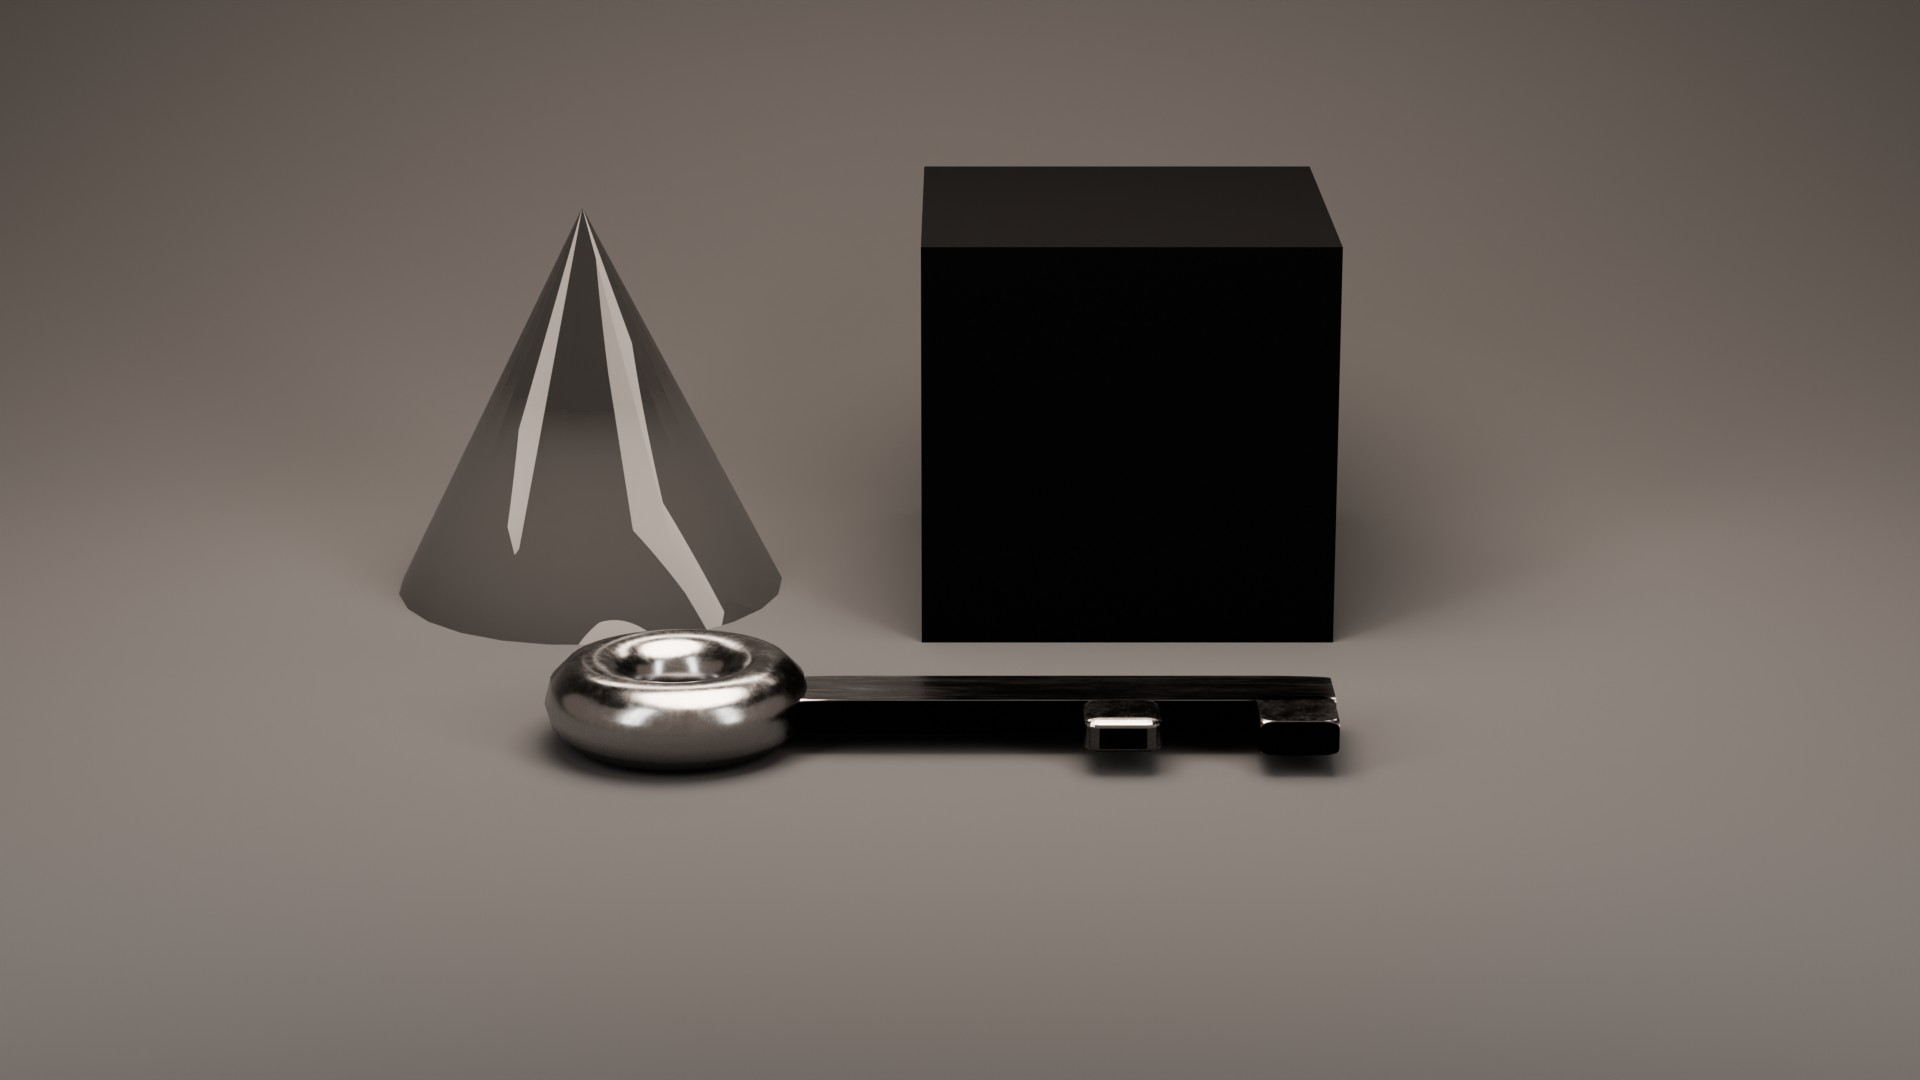
\includegraphics[width=0.5\linewidth]{img/Key.jpg}
	\caption{Glas, Metall und absorbierendes Material.}
	\label{fig:key}
\end{figure}


Im zweiten Bild wurden ausschließlich Bälle verwendet, um zu veranschaulichen, wie die verschiedenen Materialen am gleichen Objekt aussehen (siehe \autoref{fig:ball}). So entsteht eine bessere Vergleichbarkeit zwischen den verschiedenen Materialien. Außerdem kann so gezeigt werden, wie die Perspektive ebenfalls die Eigenschaften der Materialien verändern kann. Außerdem wurde beim absorbierenden Material die Farbe angepasst, um zu überprüfen, wie sehr sich die Farbwahl auf die Reflektionen auswirken.

\begin{figure}[h]
	\centering
	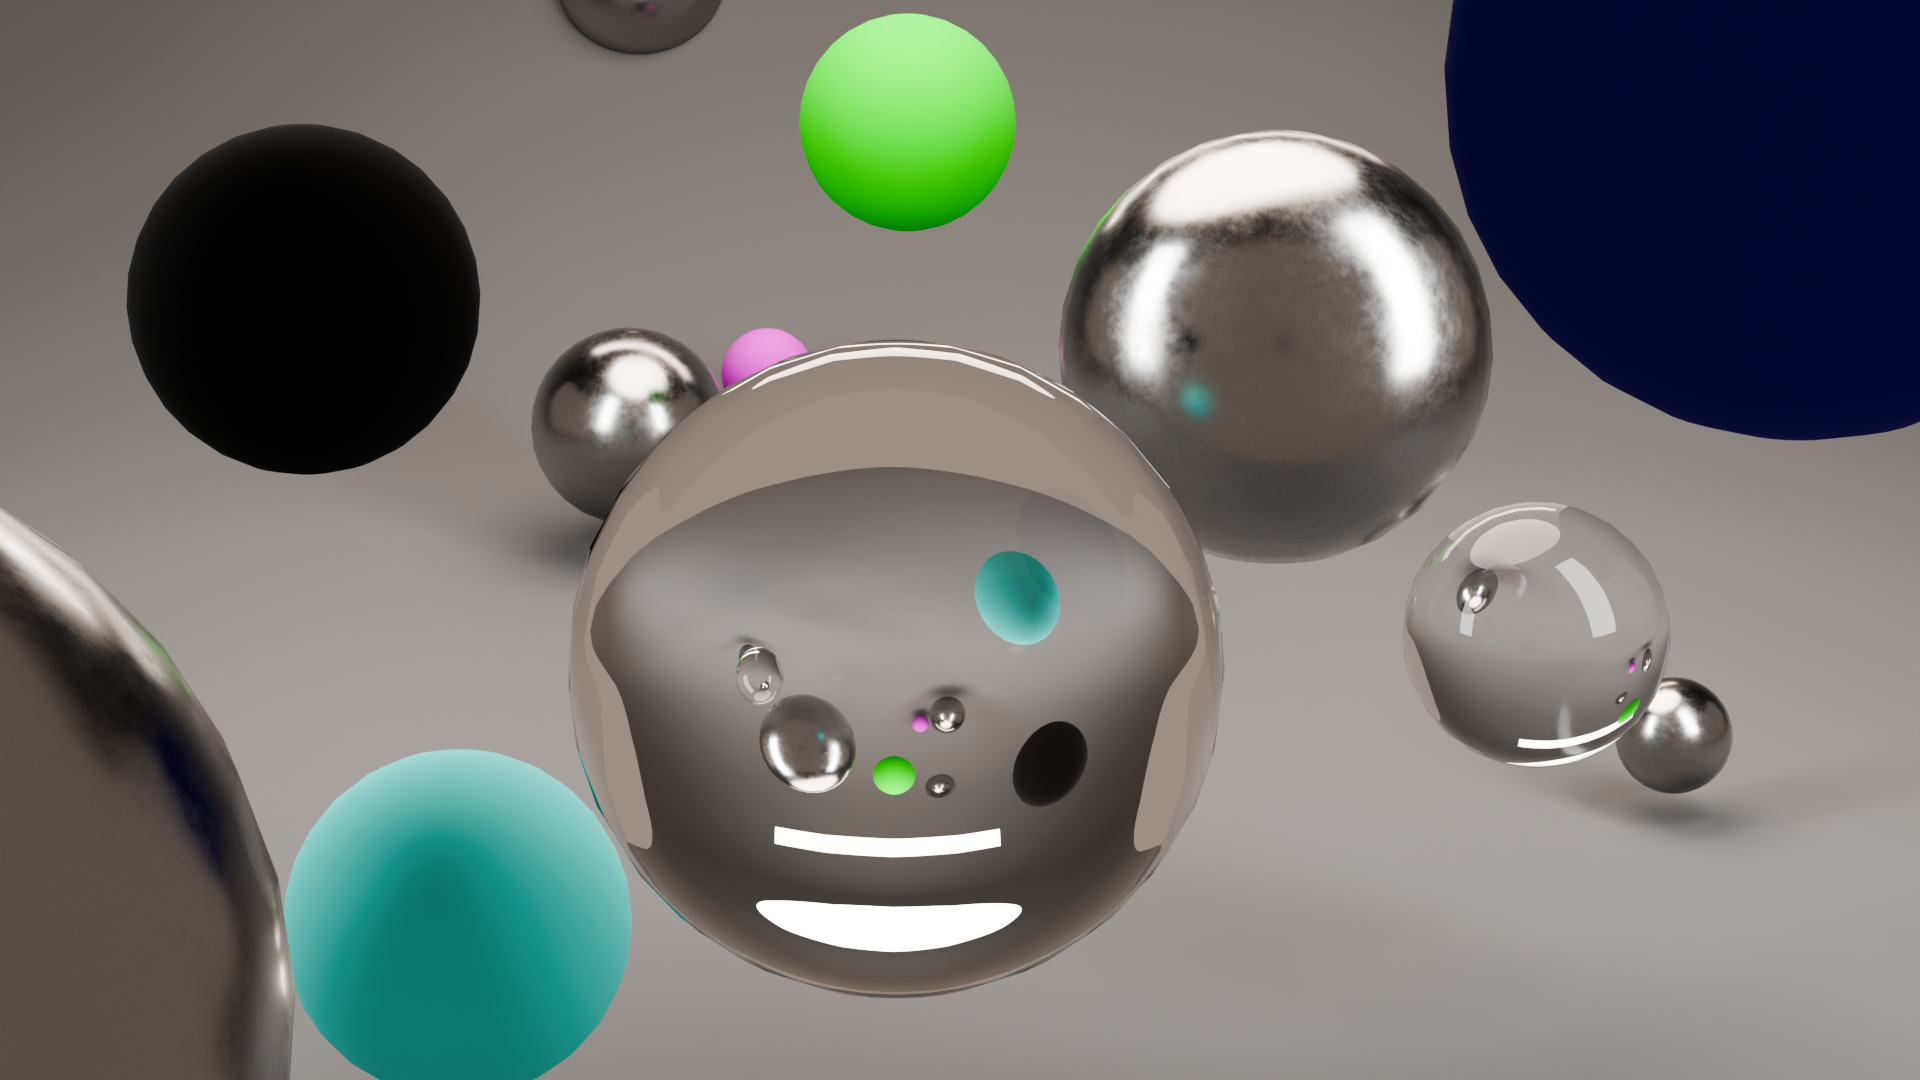
\includegraphics[width=0.5\linewidth]{img/Baelle.png}
	\caption{Kugeln mit den verschiedenen Oberflächen.}
	\label{fig:ball}
\end{figure}


\subsection{LuxCoreRender}
Die Glasoptik in Cycles kann zwar Licht durchlassen, teilweise reflektieren und die Sicht verkrümmen, allerdings war es nicht ohne weiteres möglich auch Prismeneffekte darzustellen. Deswegen wurde der LuxCoreRender benutzt, da er nicht nur Path Tracing verwendet, sondern auch zusätzliches Light Tracing. Um die Lichtbrechung darzustellen wurden zwei 3D-Dreiecke in Reihe gestellt und aus unterschiedlichen Richtungen von Lichtkegeln bestrahlt (siehe \autoref{fig:prisma}). In dem Bild kann gesehen werden, wie die Glasobjekte einen regenbogenartigen Prismaeffekt ausstrahlen. Versehentlich wird eine weitere Lichtquelle von hinten angestrahlt, weswegen sie als schwarze Raute mittig im Bild zu sehen ist. Allerdings hat der Renderprozess über 22 Stunden gedauert, weswegen kein neuer Renderversuch gestartet wurde.

\begin{figure}
	\centering
	\includegraphics[width=0.5\linewidth]{img/Prisma.png}
	\caption{Realistische Lichtbrechung von Prismen.}
	\label{fig:prisma}
\end{figure}

\section{Unity}
\label{sec:Unity}
Unity ist eine Laufzeit- und Entwicklungsumgebung für Videospiele, wird aber für die Entwicklung verschiedener 3D-Grafik-Anwendungen genutzt. In Unity gibt es verschieden Render Pipelines, wie zum Beispiel die Universal Render Pipeline (URP), die eine hohe Kompatibilität mit anderen Plattformen ermöglicht, oder die High Definition Render Pipeline (HDRP), welche eine detaillierte und hochauflösende Grafik unterstützt. Die HDRP ermöglicht auch Realtime Ray Tracing, wenn eine kompatible Grafikkarte zur Verfügung steht. Wie in \autoref{sec:Limitationen} bereits erklärt habe ich keine kompatible Grafikkarte (siehe \autoref{fig:limitation}). Dennoch wurde die HDPR verwendet, um eine möglichst realistische Annäherung zu versuchen.

\begin{figure}[h]
	\centering
	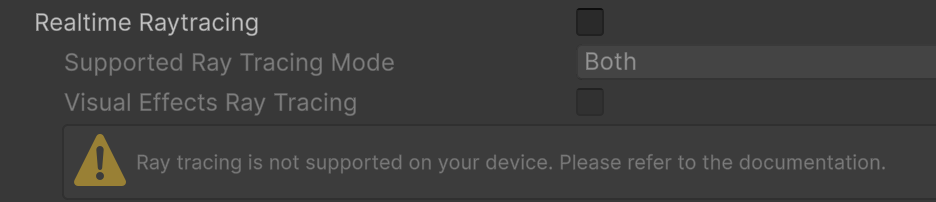
\includegraphics[width=0.5\linewidth]{img/Limitation.png}
	\caption{Ray Tracing  wird von der vorhanden Hardware nicht unterstützt.}
	\label{fig:limitation}
\end{figure}

Im weiteren Verlauf wird auf die verschiedenen implementierten Features des 3D-Labyrinths in Unity eingegangen.

\subsection{Labyrinth-Parser}
Wie in der Aufgabenstellung gefordert ist es möglich, dass das Labyrinth mithilfe eines zweidimensionalen Plans erstellt werden kann. In diesem Beispiel muss der Plan als ASCII-Datei vorliegen und aus diesen vordefinierten Zeichen bestehen:

\begin{center}
	\begin{tabular}{|l|l|}
		\hline
		\# & Mauer in Ziegelstein-Optik\\
		\hline
		G & Gläsernes Material \\
		\hline
		M & Metallisches Material\\
		\hline
		P & Spielerobjekt, welches genau ein Mal vorkommen muss\\
		\hline
		T & Zielobjekt, was maximal ein Mal vorkommen kann\\
		\hline
		. & Leeres Feld, hier befindet sich nur der Boden\\
		\hline
	\end{tabular}
\end{center}




Zusätzlich muss der Plan folgende Ansprüche erfüllen:
\begin{itemize}
	\item Jede Zeile muss genau gleich viele Zeichen enthalten, sodass immer ein rechteckiges Labyrinth entsteht
	\item Es werden nur die vordefinierte Zeichen erlaubt.
	\item Das Labyrinth muss von Mauern umrandet sein, sodass der Spieler das Spielfeld nicht verlassen kann oder nach außen blicken kann.
\end{itemize}

In dem Projekt wurde, um das Labyrinth zu laden, das selbstgeschriebene MonoBehavior-Skript \texttt{MazeLoader} verwendet. Dieses Skript erhält die entsprechenden Prefabs (und das Spielerobjekt), die dann dupliziert und an die entsprechende Stelle laut ASCII-Plan positioniert werden. Außerdem muss ein Dateipfad angegeben werden (standardmäßig liegen die Pläne in Assets/Mazes).


\subsection{Materialien}
Wie anhand der erlaubten Zeichen des Labyrinth-Parsers bereits erkennen kann, wurde trotzdem versucht die drei geforderten Materialien in Unity umzusetzen (siehe \autoref{fig:materialien}). 

Das Wandmaterial besteht aus einer einfachen Textur, die Ziegelsteinen ähnelt. Dieses Material soll das absorbierende Material darstellen, da es kaum Licht reflektiert.

Das Metallmaterial hat eine metallische Strukur, die ebenfalls als Textur hinzugefügt wurde. Außerdem wurde eine metallische Reflektion eingestellt, weswegen das Metallmaterial das reflektierende Material darstellt. Da Ray Tracing nicht aktiv ist, wird die Skybox von Unity reflektiert, unabhängig ob andere Objekte die Skybox eventuell verdecken.

Das Glasmaterial ist nahezu transparent und nur daran zu erkennen, dass je nach Perspektive die Objekte hinter dem Glas verzerrt werden.

\begin{figure}[h]
	\centering
	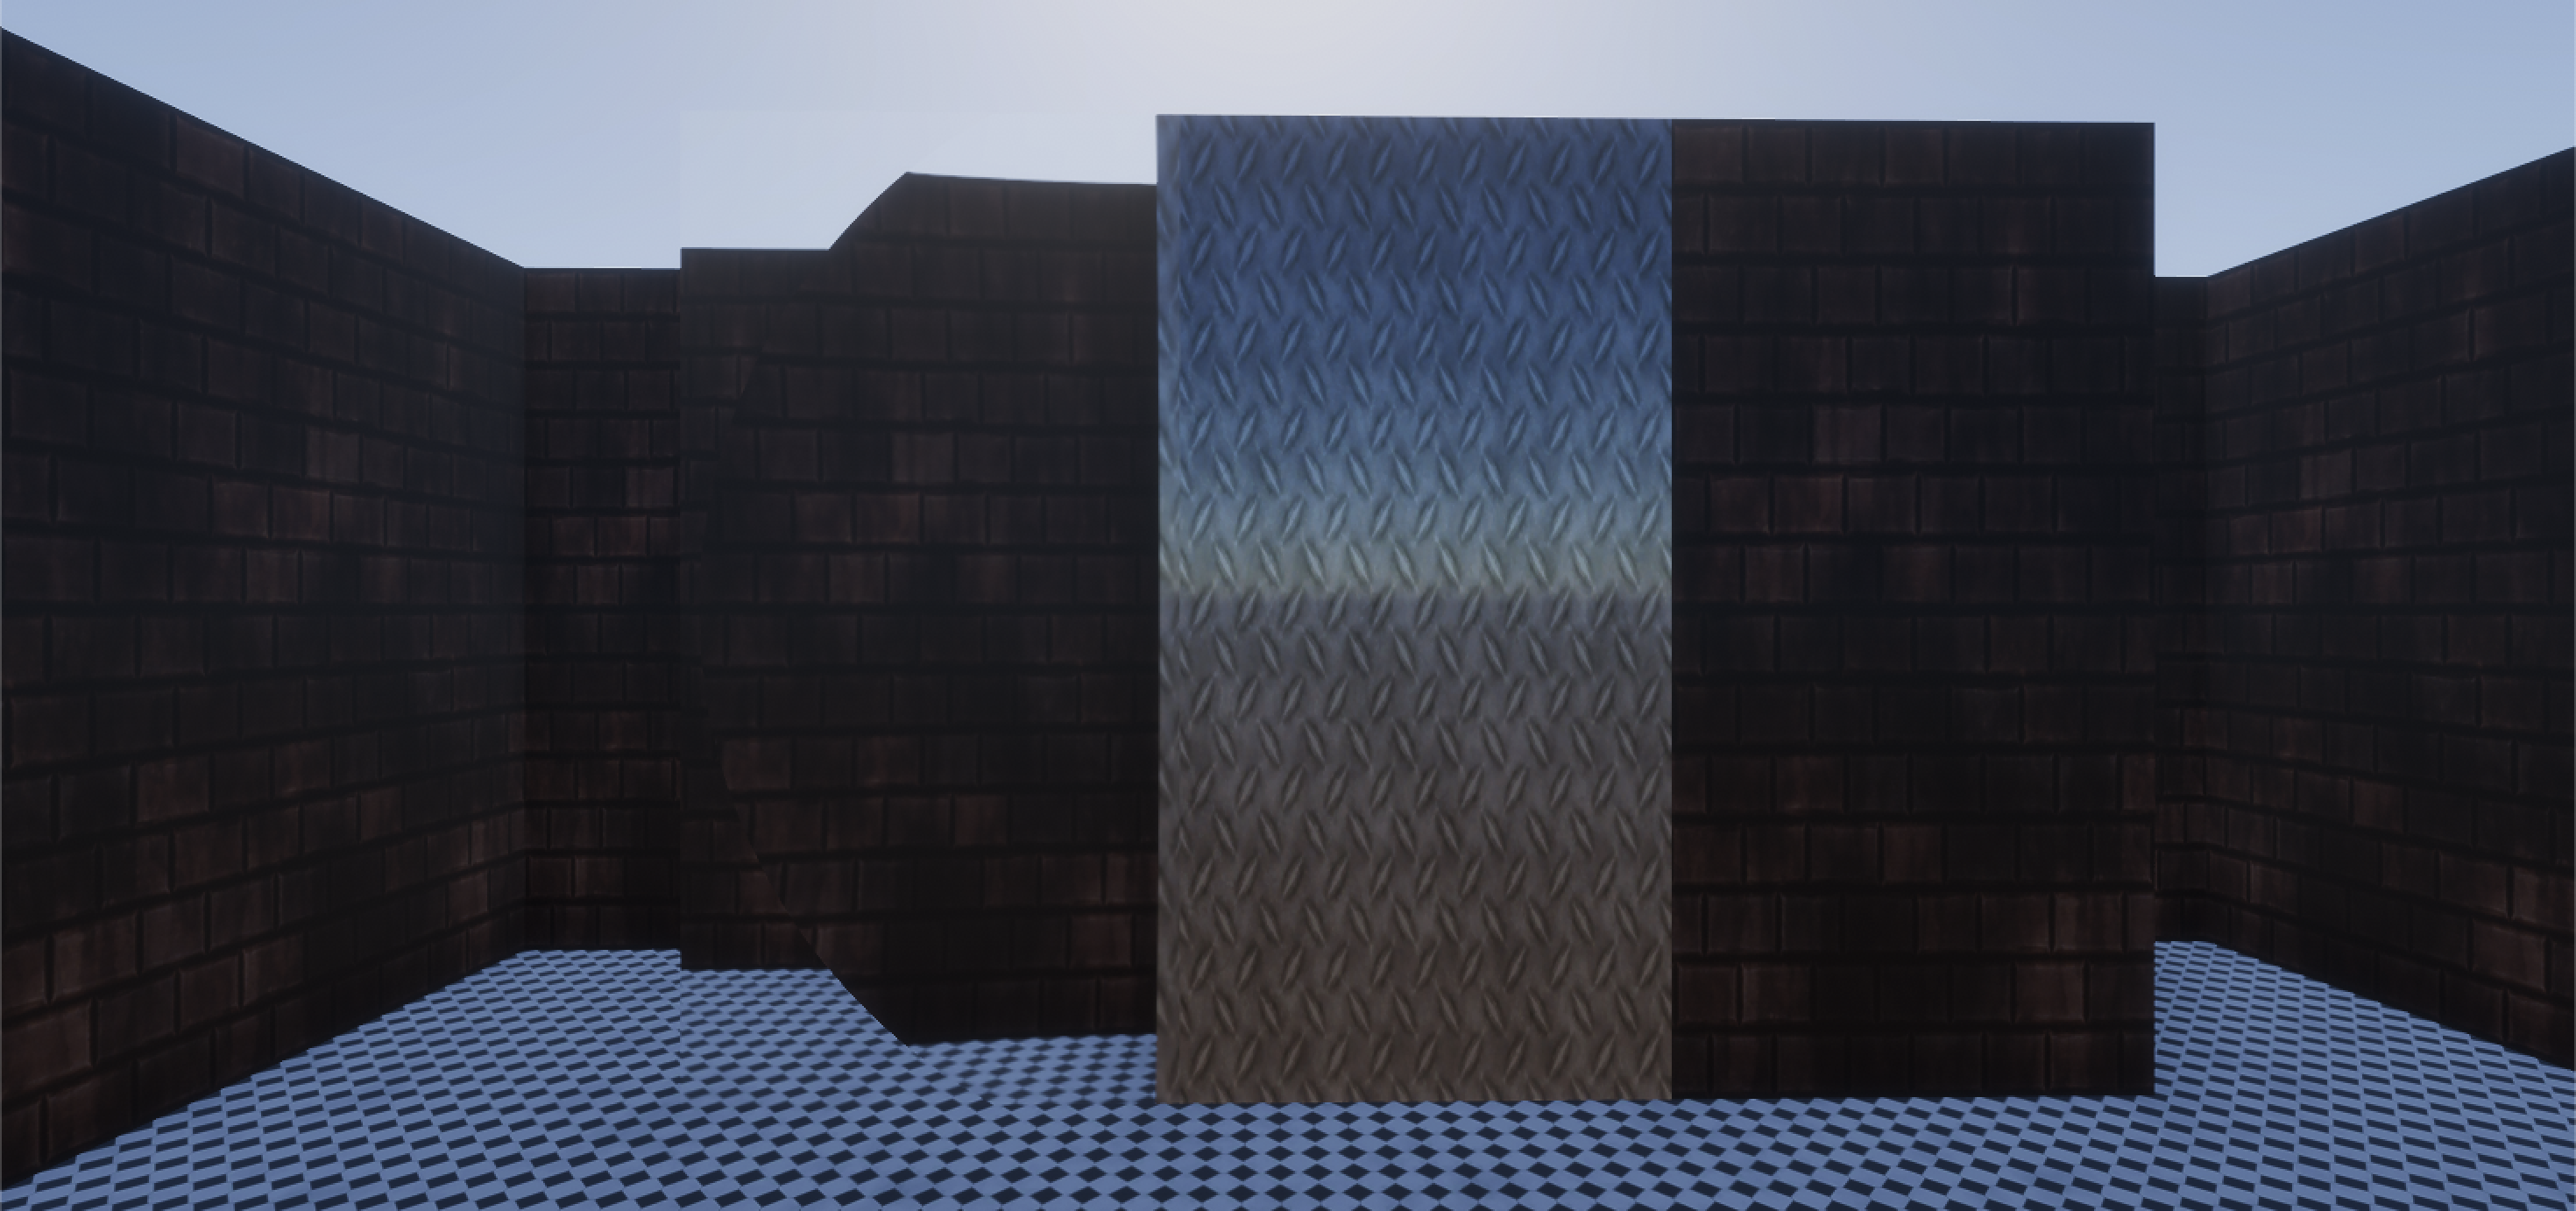
\includegraphics[width=0.5\linewidth]{img/Materialien.png}
	\caption{Screenshot aus \texttt{materialshow.txt} zur Veranschaulichungen der Materialien. Hier können das Glasmaterial (links), das Metallmaterial (mittig) und das Wandmaterial (rechts) gesehen werden.}
	\label{fig:materialien}
\end{figure}



\subsection{Steuerung}
Die Spielerbewegung basiert auf einem eigenen \texttt{PlayerController}-Skript, das mit dem Unity Input System arbeitet. Die Steuerung erfolgt in der Ego-Perspektive, mit Maus und Tastatur. Bewegt wird sich mit den Pfeiltasten, während man sich mit der Maus umsehen kann (Rotation um die y-Achse). Für die Bewegung wird das \texttt{CharacterController}-Component verwendet, das die Kollisionsabfrage und Physikbewegung übernimmt.

Die Eingaben werden über PlayerInput empfangen und an die Methoden \texttt{OnMove()} und \texttt{OnLook()} im Skript weitergeleitet. Dort werden die aktuellen Werte gespeichert und im Update()-Zyklus zur Bewegung des Spielers verwendet. 

Die Verwendung des CharacterControllers hat zum Vorteil, dass dort er auch gleichzeitig als eine Art Rigidbody und CapsuleCollider für den Spieler fungiert. Da die Wände ebenfalls einen Rigidbody besitzen wird so verhindert, dass die Objekte kollidieren können. Mit anderen Worten kann der Spieler nicht durch die Wände gehen, so wie man es bei einem Labyrinth auch erwarten würde. Außerdem kann so eine Kollision mit dem Zielobjekt erkannt werden, wodurch es dann aufgesammelt wird.


\subsection{Zielobjekt}
Das Zielobjekt sorgt dafür, dass der Spieler nicht sinnlos durch das Labyrinth irrt, sondern ein Ziel hat, nachdem gesucht werden kann. Das Zielobjekt ist eine Plane, welche eines der offline gerenderten Bilder (siehe \autoref{sec:Blender}) als Textur lädt. Dafür verwendet es das selbstgeschriebene \texttt{ImageBehavior} Skript, welches ein zufälliges Bild aus dem Ordner Assets/Rendered\_Images lädt.

Berührt der Spieler das Zielobjekt, so wird das Bild im Vollbildmodus geöffnet und kann so betrachtet werden. Der Spieler kann mit der ESC-Taste oder per Mausklick das Vollbild schließen. Während der Vollbild-Ansicht wird die Bewegung des Spielers verhindert, sodass er sich nicht versehentlich bewegt, ohne es zu merken. Das Zielobjekt wird anschließend auf inaktiv gesetzt, um es für den Nutzer als eingesammelt zu markieren. Der Ablauf wird zur leichteren Verständnis auch als UML-Sequenzdiagramm in \autoref{fig:sequenz} dargestellt.

\begin{figure}[h]
	\centering
	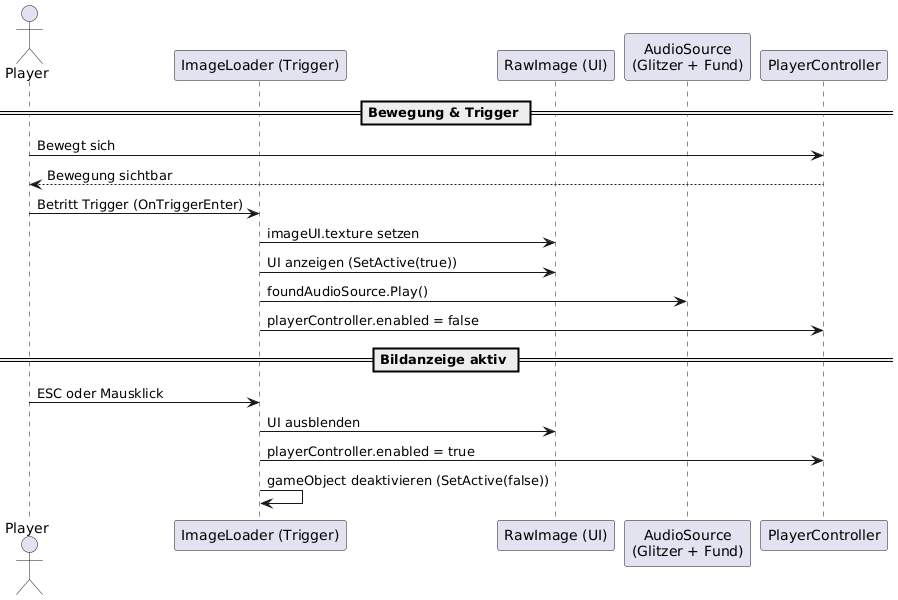
\includegraphics[width=0.7\linewidth]{img/UML.png}
	\caption{UML-Sequenzdiagramm, was den Ablauf des Einsammeln des Zielobjekts darstellt.}
	\label{fig:sequenz}
\end{figure}

\subsection{Sound}
Für eine bessere Immersion werden Sounds verwendet. Es läuft durchgängig eine Hintergrundmusik, die sich wiederholt, sobald sie endet. Es spielt auch ein kurzer Jingle, wenn der Spieler das Zielobjekt aufsammelt. Zusätzlich spielt das Zielobjekt, solange es aktiv ist, einen \glqq glitzernden\grqq\ Ton ab. Dieser wird logarithmisch lauter, je weiter sich der Spieler dem Objekt nähert. Das soll als Hilfe für den Spieler dienen, das Zielobjekt in einem großen Labyrinth zu finden. Wird der Ton leiser, so weiß der Spieler, dass er sich vom Zielobjekt entfernt.


\section{Fazit}
Das Projekt verlief in technischer Hinsicht nicht vollständig wie ursprünglich vorgesehen. Aufgrund fehlender GPU-Unterstützung für Echtzeit-Ray Tracing musste auf eine alternative Lösung zurückgegriffen werden, bei der interaktive Elemente in Unity realisiert wurden, während Ray Tracing-Bilder mit Blender (Cycles und LuxCoreRender) offline gerendert und eingebunden wurden. Dieses Vorgehen stellte sicher, dass die Anforderungen an realistische Lichtsimulation trotz der Umstände dennoch erfüllt werden konnten.

Die technische Umsetzung in Unity beinhaltete unter anderem ein ASCII-basiertes Labyrinth-Parsing, die Darstellung unterschiedlicher Materialtypen mit HDRP, interaktive Spielersteuerung, sowie eine Trigger-gestützte Bildanzeige mit Audiofeedback. Die Verwendung des neuen Unity Input Systems sowie der strukturierte Einsatz von Audioquellen, Triggern und UI-Komponenten ist eine interessante Verknüfung der verschiedenen Aspekte der Softwareentwicklung.

Mit besserer Hardware oder mehr Entwicklungszeit wäre eine Echtzeit-Ray Tracing Integration innerhalb von Unity denkbar gewesen. Die gewählte Herangehensweise zeigt jedoch, dass auch unter technischen Einschränkungen funktionale und überzeugende Ergebnisse erreichbar sind.

Alle verwendeten externen Ressourcen und Assets sind in der README.md verlinkt.



\end{document}
